\documentclass{beamer}
%\usepackage[utf8]{inputenc}
\usepackage{graphicx}
%\usepackage{tgtermes} 
\graphicspath{ {images/} }
\usepackage{mathtools}
\usepackage{amssymb}
\usepackage{amsfonts}
\usepackage{fancyvrb}
\usepackage{tikz}
\usepackage{tikz-qtree}
\usepackage{listings}
\usepackage{multicol}
\usepackage{amsthm}
\usepackage{amsmath }
\usepackage{xcolor}
\usepackage{framed}
\usepackage{color,soul}
\usepackage{tikz-cd}
\usetikzlibrary{matrix,arrows,decorations.pathmorphing, shadows, trees}
\usepackage{nomencl}
\usepackage{geometry}
\usepackage{setspace}
\usepackage{enumerate}



\theoremstyle{definition}
\newtheorem{proposition}{Proposition}
\newtheorem*{proposition*}{Proposition}
\newtheorem{definition_proposition}{Definition-Proposition}
\newtheorem*{definition_proposition*}{Definition-Proposition}
\newtheorem*{lemma*}{Lemma}
\newtheorem*{definition*}{Definition}
\newtheorem{conjecture}{Conjecture}

\title{Valuative capacity of compact subsets of ultrametric spaces}
\author{Anne Johnson}
\date{August 9, 2019}



\begin{document}
\maketitle

\begin{frame}{Background}
\begin{definition}	
(\cite{fek}) Let $K \subseteq \mathbb{C}$ be a compact subset. Fix $n \in \mathbb{N}$, and for $z = (z_1,\ldots,z_n) \in K^n$, consider
\[\delta_n(z) = \prod_{j < i} \lvert z_i - z_j \rvert^{\frac{2}{(n(n-1))}} \]
An element $z = (z_1,\ldots,z_n) \in K^n$ is called a \textbf{Fekete n-tuple} if $z$ maximizes $\delta_n$ over all $n-$tuples in $K$.
\end{definition}
%Note to self: do an example with 5 charged particles in a conductor
%Note to self: this cannot be done recursively
\end{frame}

\begin{frame}{Background}
	\begin{definition}	
		\cite{fek} Let $K$ be a compact subset of a metric space, $(M,\rho)$. Fix $n \in \mathbb{N}$, and for $z = (z_1,\ldots,z_n) \in K^n$, consider
		\[\delta_n(z) = \prod_{j < i} \rho(z_i, z_j)^{\frac{2}{(n(n-1))}} \]
		An element $z = (z_1,\ldots,z_n) \in K^n$ is called a \textbf{generalized Fekete n-tuple} if $z$ maximizes $\delta_n$ over all $n-$tuples in $K$.
	\end{definition}
\end{frame}

\begin{frame}{Background}
 \begin{definition}
		(\cite{mb1}) Let $S$ be a subset of $\mathbb{Z}$  and let $p$ be any prime. A \textbf{$p$-ordering} of $S$ is a sequence, $\{a_i\}_{i\geq 0}$ in $S$, such that $a_0$ is arbitrary and for $i >0$, $a_i$ minimizes 
		\[ v_p (\prod_{j < i} (z - a_j) )\] over $z \in S$.\\
 \end{definition}
	\pause
 \begin{itemize}
		\item $p-$orderings give a recursive construction for generalized Fekete $n-$tuples\only<+>{.}\only<+->{!}  
 \end{itemize}	
\end{frame}

\begin{frame}{Background}
\begin{definition}	
	(\cite{fek})Let $K \subseteq \mathbb{C}$ be a compact subset. The \textbf{transfinite diameter} of $K$ is \[ \lim_{n\to\infty} [ \max_z \text{ } \delta_n(z)]\] where the maximum is taken over all $n-$tuples in $K$. %That is, the transfinite diameter of $K$ is $ \lim_{n\to\infty} \delta_n(z)$, where $z$ is a Fekete $n-$tuple for each $n$.
\end{definition}
%Note to self: the convergence of this expression is Fekete's lemma
\end{frame}

\begin{frame}{Background}
\begin{proposition*}
	(\cite{jlc}, theorem 4.2)	Let $E$ be a subset of $V$, a rank-one valuation domain with valuation $v$. If $\{a_i\}_{i \geq 0}$ is $v-$ordering of $E$, then
	\[\lim_{n\to\infty} \frac{1}{n} \sum_{k=0}^{n-1} v(a_n-a_k) =\frac{2}{n(n+1)} \inf_{x_0, \ldots, x_n \in E} v (\prod_{0\leq j < i \leq n} (x_i-x_j))\]
\end{proposition*}
\end{frame}

\begin{frame}{Valuative capacity: set-up}
	\begin{definition}
		(\cite{kj}) Let $S$ be a compact subset of $(M,\rho)$. A \textbf{$\rho$-ordering} of $S$ is a sequence, $\{a_i\}_{i\geq 0}$ in $S$, such that $a_0$ is arbitrary and for $i >0$, $a_i$ maximizes 
		\[ \prod_{j < i} \rho(z, a_j) )\] over $z \in S$.\\
	\end{definition}
	\pause
    \begin{itemize}
	   \item If $\rho$ is an ultrametric, the terms $\prod_{i=0}^n \rho(a_n - a_j)$ do not depend on the choice of $\rho-$ordering. We call this the \textbf{$\rho-$sequence} of $S$. \\
	\end{itemize}
\end{frame}

\begin{frame}{Valuative capacity: set-up}
	\begin{itemize}
		\item $\rho-$orderings give a recursive construction for generalized Fekete $n-$tuples.\\	
		\pause	
		\item The limit \[ \omega(S):= \lim_{n\to\infty} [\prod_{i=0}^n \rho(a_n - a_j)]^{\frac{1}{n}}\] is called the \textbf{valuative capacity} of $S$.
	\end{itemize}		  
\end{frame}

\begin{frame}{Valuative capacity: facts}
Valuative capacity has the following properties:
\begin{itemize}
	\item \textit{translation-invariance}, i.e., $\omega(a+S) = \omega(S)$\\ (under a translation-invariant operation)
	\pause
	\item \textit{scaling}, i.e., $\omega(bS) = \lvert b\rvert \omega(S)$\\ (under a multiplicative norm)
	\pause
	\item \textit{decomposition}, i.e., \[\frac{1}{log(\frac{\omega(S)}{d}) } = \sum_{i=1}^n \frac{1}{log(\frac{\omega(A_i)}{d})}\]
	for $d=diam(S)$ and $\rho(A_i, A_j)=d, \forall i,j$ 
\end{itemize}	
\end{frame}

\begin{frame}{Recursive $\rho-$orderings}
	\tikzset{font=\tiny,
	level distance=1.35cm,
}

\begin{center}
	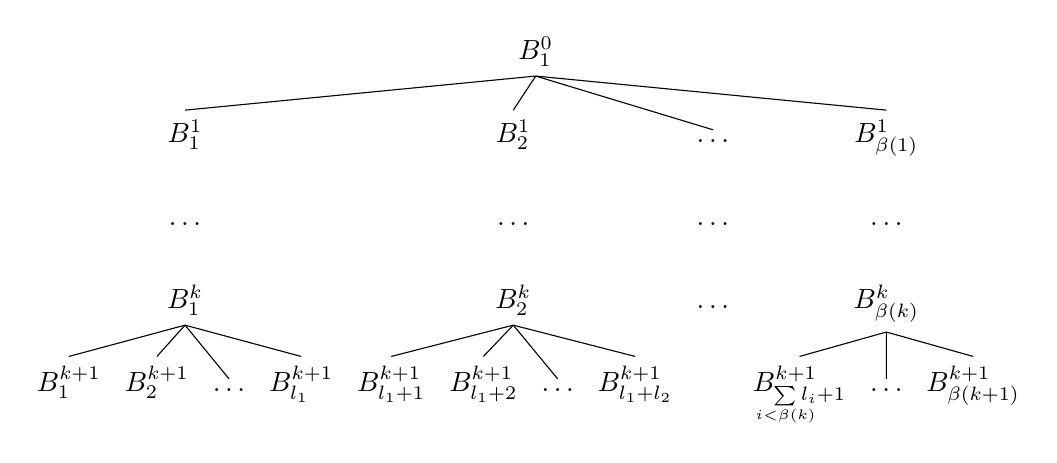
\begin{tikzpicture}
\Tree [. $B^0_1$ [. $B^1_1$ \edge [draw=none]; [. $\ldots$ \edge [draw=none]; [. $B^k_1$ [. $B^{k+1}_1$ ] [. $B^{k+1}_2$ ]  [. $\ldots$ ] [. $B^{k+1}_{l_1}$ ] ] ] ] 
[. $B^1_2$ \edge [draw=none]; [. $\ldots$ \edge [draw=none]; [. $B^k_2$ [. $B^{k+1}_{l_1 + 1}$ ] [. $B^{k+1}_{l_1 + 2}$ ] [. $\ldots$ ] [. $B^{k+1}_{l_1 + l_2}$ ] ] ] ] 
[. $\ldots$  \edge [draw=none]; [. $\ldots$ \edge [draw=none]; [. $\ldots$ ] ] ]
[.$B^1_{\beta(1)}$ \edge [draw=none]; [. $\ldots$ \edge [draw=none]; [.$B^k_{\beta(k)}$ [. $B^{k+1}_{\sum\limits_{\mathclap{i < \beta(k)}}  l_i + 1 }$ ] [. $\ldots$ ] [. $B^{k+1}_{\beta(k+1)}$ ] ] ] ] ]
\end{tikzpicture}
\end{center}
\end{frame}

\begin{frame}{Recursive $\rho$-orderings}
	
%Note to self: write notation on the board, $\Gamma_S$ and $\beta(k)$

	\begin{itemize}
		\item $\rho_{k+1}-$ordering of $S_{\gamma_{k+1}}$ is found by selecting elements of each $B^k_i$ in order as much as possible, and skipping to $B^k_{i+1}$, when it is not possible.
		\pause
		\item  to build a $\rho-$ordering of $S$ from the above, it suffices only to make a choice of centres for each of $B^k_i$'s.
	\end{itemize}
%Note to self: talk about shuffles
\end{frame}


\begin{frame}{Semi-regularity}
%Note to self: define semi-regularity	
\begin{proposition}
	If $S$ is a semi-regular ultrametric space, $\delta$ is the characteristic sequence of $S$, $\beta$ is the structure sequence of $S$, and $\alpha$ is the sequence describing the semi-regularity, then
	\[v_{\gamma_k}(\delta(n)) =  \lfloor\frac{n}{\beta(k)}\rfloor - \lfloor\frac{n}{\beta(k+1)}\rfloor = \sum_{j=1}^{\alpha(k)-1} \lfloor \frac{n + j\cdot \beta(k)}{\alpha(k)\beta(k)} \rfloor\]
\end{proposition}

\end{frame}


\begin{frame}{Regularity}
	%Note to self: define regularity
\begin{proposition}
	Let $S$ be a regular, tame subset of a compact ultrametric space with $\gamma_k = q^{c_k}$ for some $c_k \in \mathbb{Q}$ and for all $k \in \mathbb{N} \cup 0$. Then 
	\[v_{q}(\delta(n)) =  c_0n + \sum_{k=1}^{\infty} (c_{k} - c_{k-1}) \cdot \lfloor\frac{n}{q^{k}}\rfloor \]
	and 
	\[log_q(\omega(S)) = \lim_{n\to\infty} c_0 + \frac{1}{n}\sum_{k=1}^{\infty} (c_{k} - c_{k-1}) \cdot \lfloor\frac{n}{q^{k}}\rfloor  \]
\end{proposition}
\end{frame}

\begin{frame}
	\begin{itemize}
		\item  Semi-regularity implies the presence of a ``well-balanced" partition of $S$.
		\pause
		\item Regularity shows us that we can recover a notion of scaling, when the conditions are right.
		\pause 
		\item Taken together, they extend the toolkit for computing capacity without appealing to algebraic structure\only<+>{.}\only<+->{!} 
	\end{itemize}
\end{frame}


\begin{frame}{Product Space}
\begin{proposition}
	Let $(M_i, \rho_i)$, for $i$ in some finite index set $I$, be a collection of metric spaces and suppose $\rho_i$ is an ultrametric for each $i$. Then $(M,\rho_\infty)$ is an ultrametric space, where $M=M_1 \times M_2 \times \ldots \times M_n$ and $\rho_\infty$ is the metric described above.
\end{proposition}
\pause
\begin{itemize}
	\item Let $M=(\mathbb{Z}^n, \rho_{p, \infty})$ be the ultrametric space with points equal to the $n$-fold product of $(\mathbb{Z}, \rho_p)$ (for $n < \infty$) for some fixed prime $p$. The valuative capacity of $M$ is  $(\frac{1}{p})^{\frac{1}{p^n-1}}$.
	\pause
	\item What about primes $p \neq q$?
\end{itemize}
\end{frame}

\begin{frame}{Product Space: primes $p \neq q$}
	\begin{itemize}
		\item These spaces do not have a scaling property and they are not regular.
		\pause
		\item We use the fact that they are semi-regular and study the exponent of each prime in turn.
	\end{itemize}
\end{frame}

\begin{frame}{Product Space: $(\mathbb{Z},\rho_2) \times (\mathbb{Z},\rho_3)$}
\begin{lemma}
	Let $S = (\mathbb{Z},\rho_2) \times (\mathbb{Z},\rho_3) $ and consider the $k^{th}$ element of the $\beta$ sequence of $S$, $\beta(k) = 2^i \cdot 3^j$. If $k$ is such that $\gamma_k=2^{-i}$ for some $i$, then $j$ counts the numbers $a \in \mathbb{Z}_{\geq 0}$ such that $3^a < 2^{i}$.
\end{lemma}
\pause
\begin{proof}
	\begin{itemize}
	\item $\Gamma_S$ is strictly monotone decreasing and each $\gamma_k$ is equal to a non-positive power of $2$ or $3$. \pause
	\item If $\gamma_k = 2^i$, then all non-positive powers of $3$ and $2$ which are greater than $2^i$ must be equal to some $\gamma_j$, $0 \leq j < k$.\pause %That is, $2^i$ only appears in the $\Gamma_S$ sequence after all larger powers of $2$ and $3$ have been exhausted.
	\item Since we are only considering the case $\gamma_k$ is a power of $2$, this includes all of the smaller powers of $3$.
	\end{itemize}
\end{proof}
\end{frame}
\begin{frame}{Product Space: $(\mathbb{Z},\rho_2) \times (\mathbb{Z},\rho_3)$}
	 \[v_{\gamma_{\frac{1}{2}}}(\delta(n)) = \sum_{i=1}^\infty i \cdot \lfloor\frac{n + 2^i \cdot 3^{\lceil \frac{i}{log_2(3)}\rceil}}{2^{i+1}\cdot 3^{\lceil \frac{i}{log_2(3)}\rceil}} \rfloor\]
		\pause
	 \[v_{\gamma_{\frac{1}{3}}}(\delta(n)) = \sum_{i=1}^\infty i \cdot (\lfloor\frac{n + 2^{\lceil \frac{i}{log_3(2)}\rceil} \cdot 3^i}{2^{\lceil \frac{i}{log_3(2)}\rceil}\cdot 3^{i+1}} \rfloor + \lfloor\frac{n + 2^{\lceil \frac{i}{log_3(2)}\rceil+1} \cdot 3^i}{2^{\lceil \frac{i}{log_3(2)}\rceil}\cdot 3^{i+1}} \rfloor) \]
\end{frame}

\begin{frame}{Product Space: primes $p \neq q$}
\begin{conjecture} Finite products of $(\mathbb{Z}, \rho_{p_i})$ for distinct primes, $p_i$, have transcendental valuative capacity.\\ \end{conjecture}
\end{frame}


\begin{frame}
\frametitle{references}
\begin{thebibliography}{9}
%	\bibitem[Ac]{na} N.L. Ackerman, Completeness in Generalized Ultrametric Spaces, \textit{$p$-Adic Numbers, Ultrametric Analysis, and Applications} \textbf{5(2)} (2013), 89-105.
%	\bibitem[Am]{amice} Y. Amice, Interpolation $p$-adique, \textit{Bull. Soc. Math. France} \textbf{92} (1964) 117-180.
%	\bibitem[BR]{rum} M. Baker and R Rumely, \textit{Potential Theory and Dynamics on the Berkovich
%		Projective Line}, Amer. Math. Soc., Providence, 2010.
	\bibitem[B1]{mb2} M. Bhargava, $P$-orderings and polynomial functions on arbitrary subsets of Dedekind
	rings, \textit{J. reine angew. Math.}, \textbf{490} (1997), 101-127.
	\bibitem[B2]{mb1} M. Bhargava, The factorial function and generalizations, \textit{Am. Math. Monthly}
	\textbf{107} (2000), 783-799.
%	\bibitem[B3]{mb3} M. Bhargava, On $P$-orderings, Rings of Integer Valued Polynomials and Ultrametric
%	Analysis, \textit{Journal of the Amer. Math. Soc.} \textbf{22(4)} (2009), 963-993.
%	\bibitem[Ca]{dgc}  D. Cantor, On an extension of the definition of transfinite diameter and some applications, \textit{J. reine angew. Math} \textbf{316} (1980), 160-207.  
	\bibitem[Ch]{jlc} J.-L. Chabert, Generalized factorial ideals, \textit{Commutative algebra, Arab. J. Sci. Eng.
		Sect. C} \textbf{26} (2001), 51-68.
%	\bibitem[CEF]{cef} J.-L.Chabert, S. Evrard, Y. Fares, Regular subsets of valued fields and Bhargava’s $v$-orderings, \textit{Math. Z.} \textbf{274} (2013) 263-290.
%	\bibitem[EF]{ef} S. Evrard and Y. Fares, $p$-adic subsets whose factorials satisfy a generalized Legendre
%	formula, \textit{London Math. Soc.}, \textbf{40} (2008), 37-50.
%	\bibitem[FP]{fp} Y. Fares, S. Petite, The valuative capacity of subshifts of finite type, \textit{J. Number Theory} \textbf{158}
%	(2016), 165-184.
	%\bibitem[GV]{gvdp} Lothar Gerritzen and Marius van der Put, Schottky Groups and Mumford Curves.
	\bibitem[F]{fek} M. Fekete, Uber die Verteilung der Wurzelen bei gewisser algebraiche Gleichun-
	gen mit ganzzahligen Koeffizienten, \textit{Math. Zeits.} \textbf{17} (1923), 228-249.
	\bibitem[J1]{kj} K. Johnson, $p$-orderings, Fekete $n-$tuples and capacity in ultrametric spaces (in preparation).
%	\bibitem[J2]{kj2} K. Johnson, Limits of characteristic sequences of integer-valued polynomials on
%	homogeneous sets, \textit{J. Number Theory} \textbf{129} (2009), 2933-2942.
%	\bibitem[M]{mun} J. Munkres, \textit{Topology}, Prentice Hall Inc., Upper Saddle River NJ, 2000.
%	\bibitem[Ra1]{rand} T. Ransford, \textit{Potential Theory in the Complex Plane}, Cambridge University Press, Cambridge, 1995.
%	\bibitem[Ra2]{rand2} T. Randsford, Computation of Logarithmic Capacity, \textit{Comp. Methods Function Theory} \textbf{10} (2010), 555-578.
%	\bibitem[Ro]{ar} A.M. Robert, \textit{A course in p-adic analysis}, Springer-Verlag, New York, 2000.
%	\bibitem[S]{sim} B. Simon, Equilibrium measures and capacities in spectral theory, \textit{Inverse Probl. Imaging} \textbf{1}:4 (2007), 713–772. 
%	\bibitem[W]{wer} J. Wermer, \textit{Potential Theory}, Springer Lecture Notes in Mathematics, \textbf{408}, Providence, 1981.
\end{thebibliography}\end{frame}

\end{document}